\section{Experimental Data}

    We generated several problem suites with \fuzzer{} that made one solver perform poorly, but not others. The graphs in the figures below show the performance results. All experiments were run in series on the same Linux computer, with a timeout of 15 seconds.

    \begin{figure}[H]
        \begin{subfigure}{.5\textwidth}
            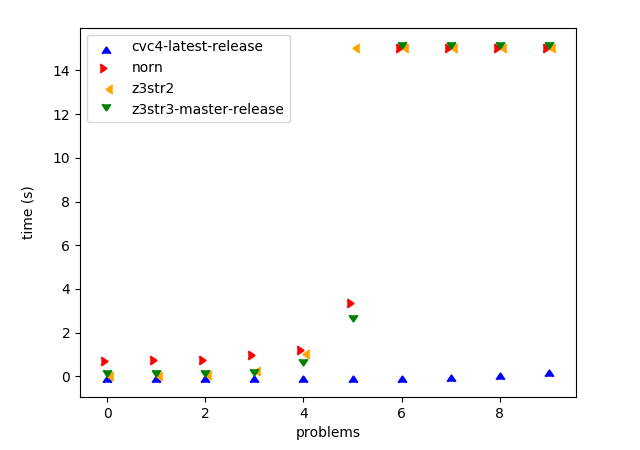
\includegraphics[width=\textwidth]{data/graphs/concats-balanced.png}
            \label{fig:concats-balanced}
            \caption{Performance on concats-balanced}
        \end{subfigure}
        \begin{subfigure}{.5\textwidth}
            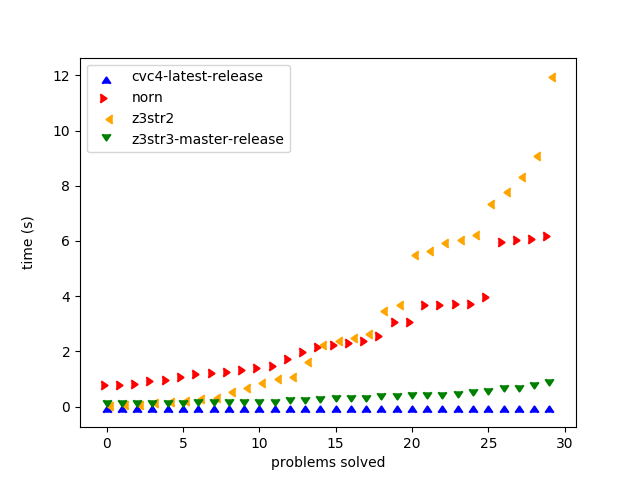
\includegraphics[width=\textwidth]{data/graphs/concats-small.png}
            \label{fig:concats-small}
            \caption{Performance on concats-small}
        \end{subfigure}
        \begin{subfigure}{.5\textwidth}
            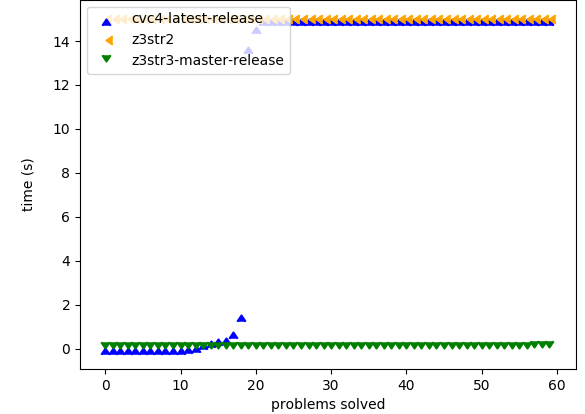
\includegraphics[width=\textwidth]{data/graphs/concats-extracts-small.png}
            \label{fig:concats-extracts-small}
            \caption{Performance on concats-extracts-small}
        \end{subfigure}
        \begin{subfigure}{.5\textwidth}
            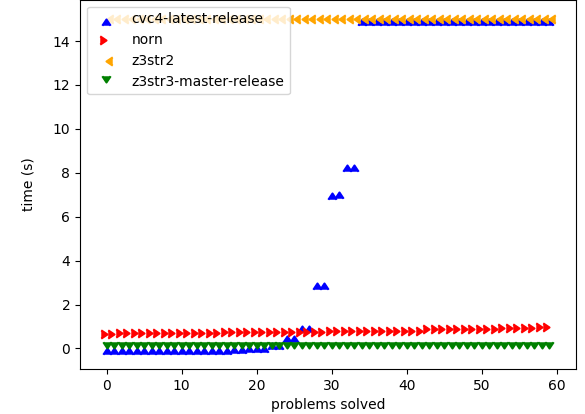
\includegraphics[width=\textwidth]{data/graphs/different-prefix.png}
            \label{fig:different-prefix}
            \caption{Performance on different-prefix}
        \end{subfigure}
        \caption{Results on selected \fuzzer{} problems}
        \label{fig:graphs}
    \end{figure}

\section{Analyses}

    In this section, we analyse the experimental results from the previous section. Although it is satisfying to find a class of problems that makes only one solver behave a certain way, it is only practically useful when the behaviour's cause is also understood.

    \todo{Maybe organise these by solver, instead of by problem?}

    \subsection{\cHard{}}

        The \cvc{} trace file suggests that it performs the following operations:

        \begin{enumerate}
            \item Loads all facts into its database.
            \item Flattens binary concatenations into n-ary concatenations.
            \item Computes equivalence classes for strings and integers.
        \end{enumerate}

        At this stage it discovers that there is a conflict in one of its equivalence classes, as shown in Figure~\ref{fig:cvc4-conflict}. After discovering the conflict, the rest of the trace is filled with apparently the same operation repeated hundreds of thousands of times. This operation dominates the content of the trace. After this expensive operation is finished, \cvc{} appears to recall the earlier conflict and returns \texttt{unsat}.

        \begin{figure}[h]
            {\scriptsize\begin{verbatim}
CONFLICT: Eq engine conflict : (and
(= "woof" (str.++ "woof" lsym_5 ... lsym_5))
(= "" lsym_5)
(= "" var3) ... (= "" var30)
(= (str.++ "woof" var3 ... var30) (str.++ "meow" var43 ... var70))
(= "" var43) ... (= "" var70)
(= "meow" (str.++ "meow" lsym_5 ... lsym_5)))\end{verbatim}}
            \caption{Evidence of \cvc{} detecting conflict}
            \label{fig:cvc4-conflict}
        \end{figure}

        \us{} behaves differently. It follows a similar process as \cvc{}, except it does not flatten concatenations. In contrast to \cvc{}, \us{} immediately returns \texttt{unsat} as soon as it verifies consistency of equivalence classes as it constructs them, as shown in Figure~\ref{fig:z3str3-conflict}.

        \begin{figure}[h]
            {\scriptsize\begin{verbatim}
-------- [str] new_eq_check ../src/smt/theory_str.cpp:1864 ---------
checking whether (str.++ "woof" var2) and (str.++ "meow" var42) can be equal
------------------------------------------------
-------- [str] new_eq_check ../src/smt/theory_str.cpp:1867 ---------
inconsistency detected: (str.++ "woof" var2) cannot be equal to (str.++ "meow" var42)
------------------------------------------------
-------- [str] assert_axiom ../src/smt/theory_str.cpp:179 ---------
asserting (not (= (str.++ "woof" var2) (str.++ "meow" var42)))
------------------------------------------------\end{verbatim}}
            \caption{Evidence of \us{} detecting conflict}
            \label{fig:z3str3-conflict}
        \end{figure}

        We were not equipped well enough to debug this behaviour in \cvc{}, but we intend this result to be useful to its authors in improving it.

    \subsection{\zHard{}}

        Both solvers exhibit similar patterns in their trace files. They differ in their strategies for assigning possible satisfying assignments.

        \todo{Explain why \us{} performs poorly.}
